\documentclass[12pt]{article}

\usepackage{graphicx}
\usepackage{paralist}
\usepackage{listings}
\usepackage{booktabs}
\usepackage{hyperref}
\usepackage[english]{babel}
\usepackage[autostyle, english = american]{csquotes}

\MakeOuterQuote{"}

\oddsidemargin 0mm
\evensidemargin 0mm
\textwidth 160mm
\textheight 200mm

\pagestyle {plain}
\pagenumbering{arabic}

\newcounter{stepnum}

\title{CAS 703 Project Report}
\author{Dong Chen}
\date{\today}

\begin {document}

\maketitle
This is the report for CAS 703 Software Design. The report will cover the implementation of 
Emfatic, Ecore, Eugenia, EVL, EOL, and model transformation.

\section{Introduction}
Typically, the state fair will be hosted in some states in the United States. In some states, 
like Iowa, Iowans host the event each year during summer. The state fair event usually will 
last for one day. During the day, participants can attend numerous events, including live shows 
and livestock competitions. Depend on how much livestock needs to manage, livestock needs a stall 
to rest. An event may also need some referees, performers, and audiences.

\section{Ecore Class Diagram}
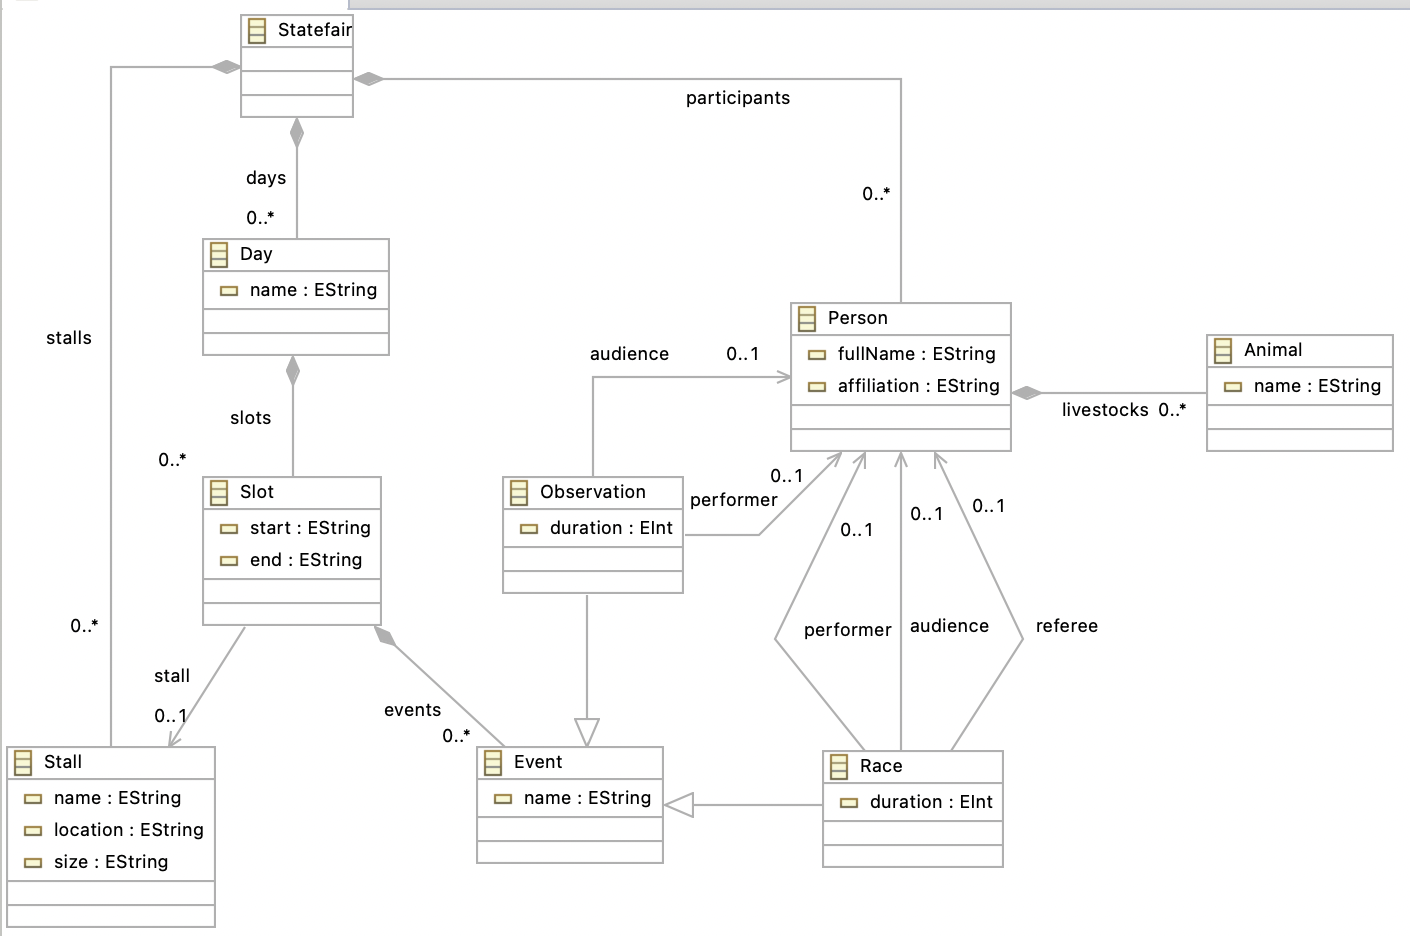
\includegraphics[scale = 0.6]{img/statefair-diagram}

\subsection{Define and Analyze Metamodel}
The following classes will be defined in Emfatic and Ecore files.
\begin{itemize}
    \item Statefair: contains multiple Person, Stall, and Day.
    \item Person: has a name, company, and multiple livestock.
    \item Day: has a name and multiple slots.
    \item Slot: has a start and end time, it also contains multiple events and a reference to Stall 
    \item Event: abstract class contains a name.
    \item Observation: has a duration, and two references to Person.
    \item Race: has a duration, and three references to Person.
    \item Stall: has a name, location, and size.
    \item Animal: has a name.
\end{itemize}

\subsection{Assumptions}
None

\subsection{Alternative Design}
An alternative way is to let the Animal class be a component of the StateFair class rather 
than a component of the Person class. 
If this is the case, in the Animal class, there would be a reference to determine who owns the livestock. 
The Observation class and Race class need to have a dependency/reference on the Animal class 
because they might require livestock in the event.

\pagebreak
\section{Concrete Syntax and Editors}
In this section, a tool called Eugenia will be implemented to create a graph editor.

\subsection{GMF and Define in Eugenia}
Eugenia helps to define the graphical modeling framework graph relationship and a new 
graph editor can be constructed.

\subsection{The Graph Editor}
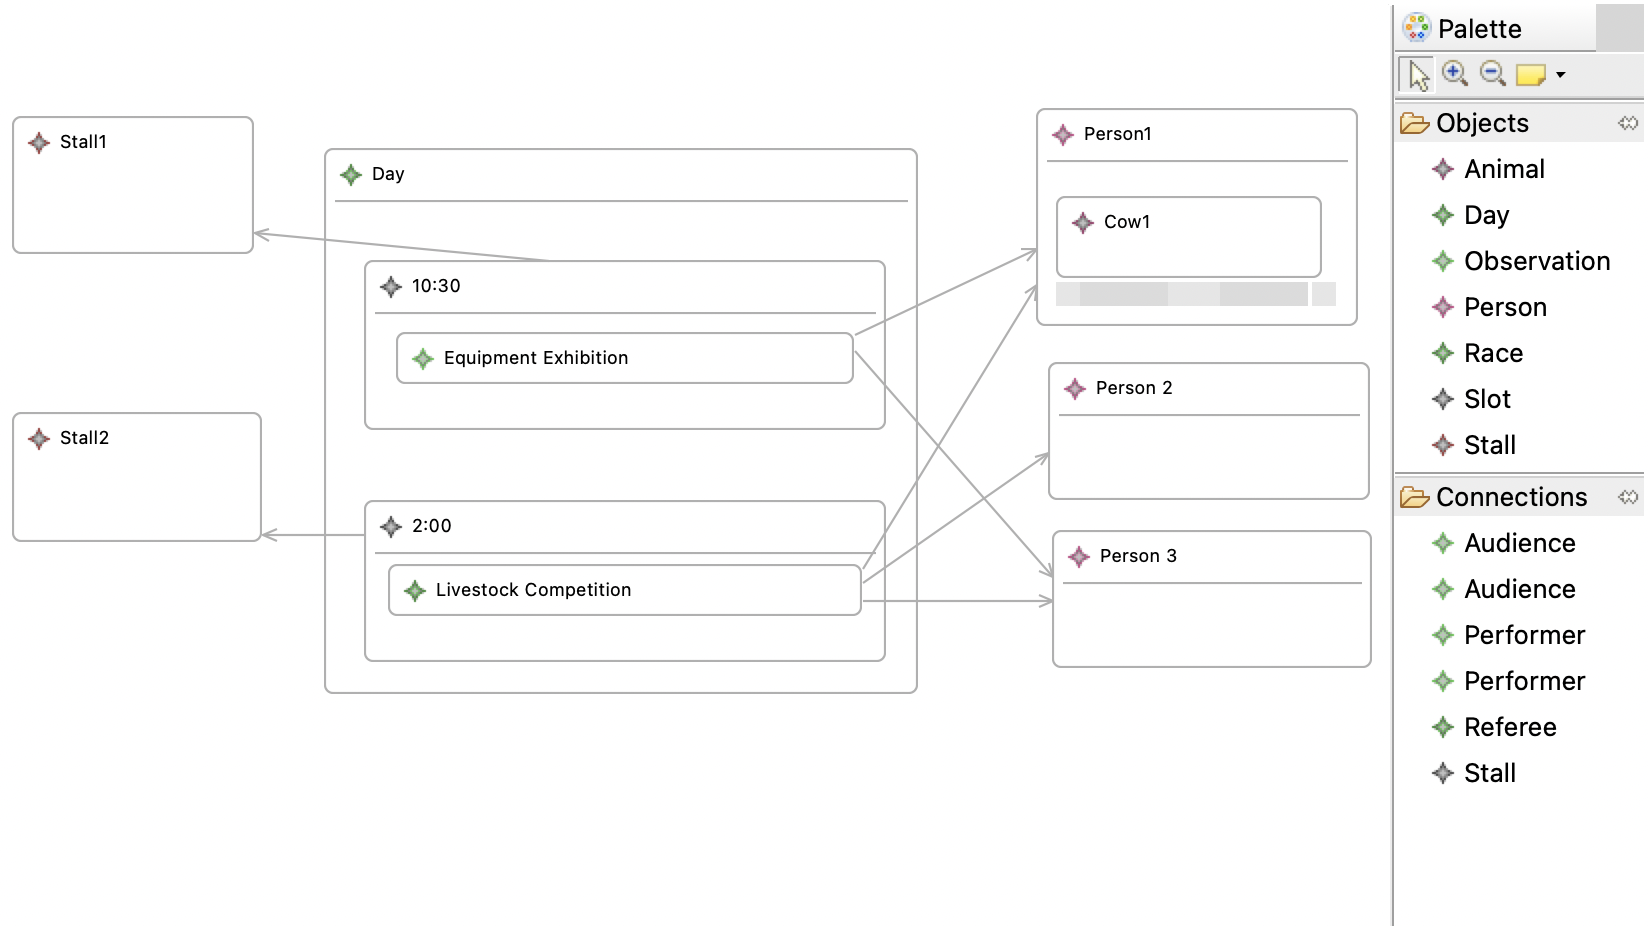
\includegraphics[scale = 0.6]{img/eugenia-editor}

The details of how to define the graph editor in the following list.

\begin{itemize}
    \item @gmf.diagram: Statefair - (this is the start of diagram)
    \item @gmf.node: Person, Day, Slot, Event(Observation, Race), Stall, Animal - (they are nodes represent each class)
    \item @gmf.link: Stall, Person - (they are dependencies/references)
    \item @gmf.compartment: Animal[*], Slot[*], Event[*] - (compartment allow a shape inside a shape)
\end{itemize}

\subsection{More Cases in the Editor}
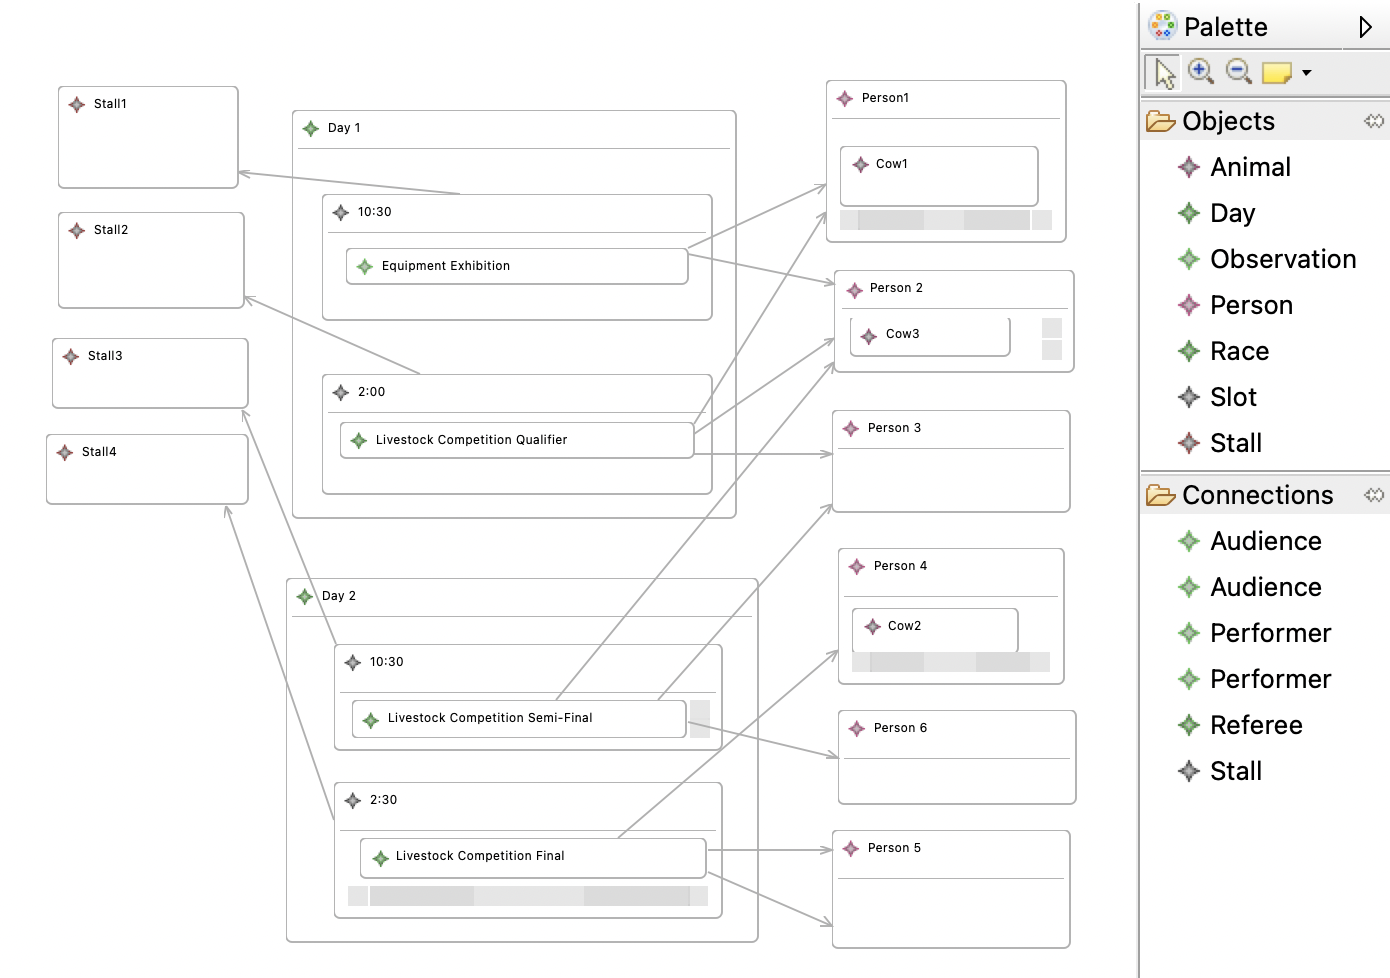
\includegraphics[scale = 0.6]{img/eugenia-editor-more}

\subsection{Strengths and Weaknesses}
\noindent \textbf{Strengths}: 
Eugenia helps to visualize the relationship between each class. It is very intuitive and easy to understand.

\noindent \textbf{Weaknesses}: 
Eventually, it can get messy when more cases add to the editor. Increased cases can lead the editor hard to read. 
Each time, it requires to launch of a new instance of the project. This is an extra step that some developers may think it is 
tedious. The work between the default eclipse and the new editor is not synchronized, which means data added in the new graph editor 
are not available in the previous tree editor.
\\Additionally, developers might feel it is inefficient to use the graph editor. 
It requires moving shapes and arrows around, and some people may get very picky on the position of each shape. A text editor can 
avoid this situation.

\pagebreak
\section{Validation Constraints}
\subsection{Queries EOL}
The following are eol queries in the StateFair.

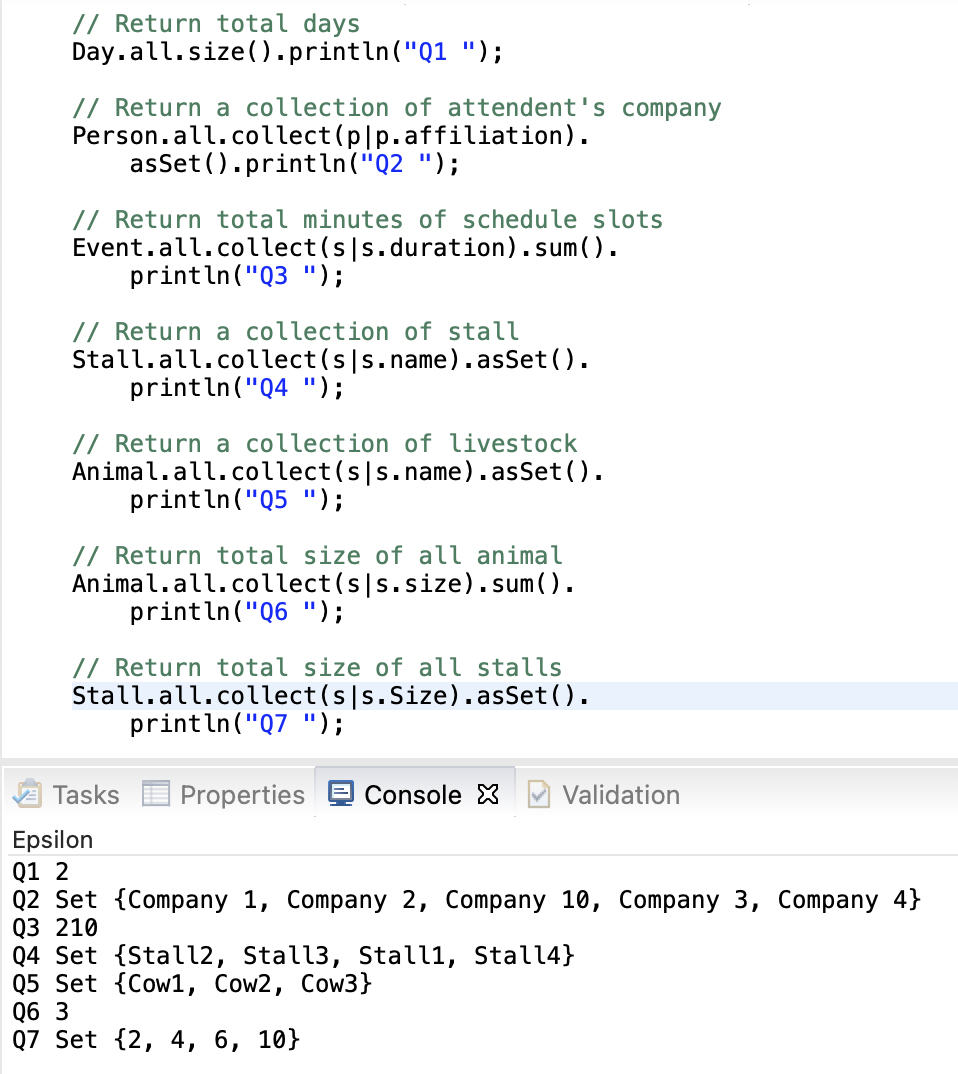
\includegraphics[scale = 0.6]{img/eol-queries}

\subsection{Constraints Analysis}
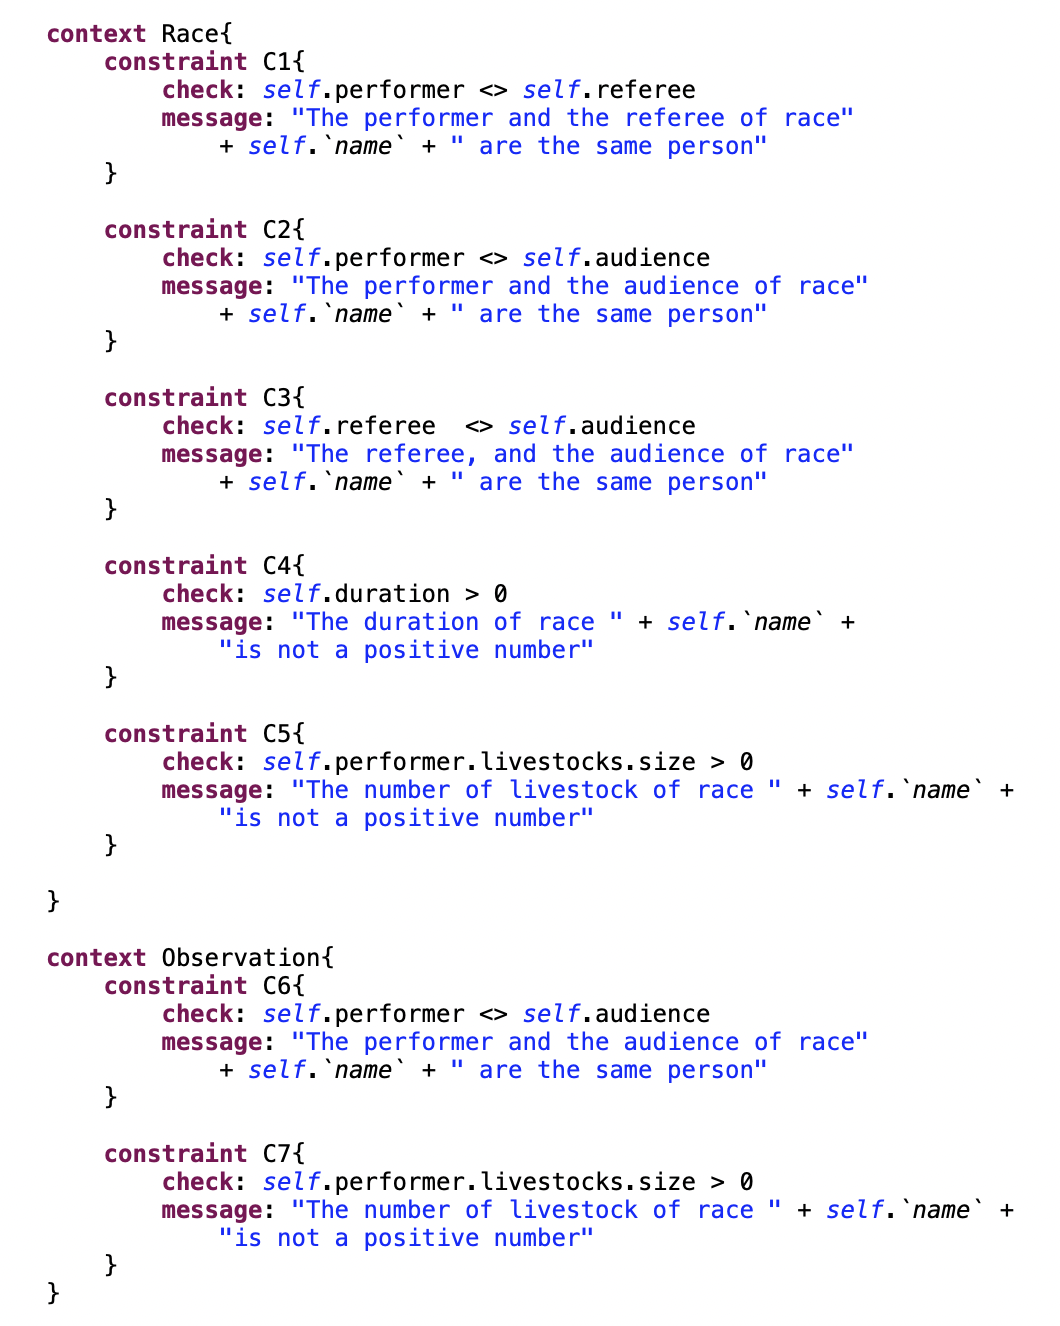
\includegraphics[scale = 0.6]{img/evl-constraints}

Firstly, there are performers, audience, and referees in the design. In most cases, these three individuals can not be the same person. 
Secondly, the duration of each event should great than 0 minutes. Thirdly, the size of livestock should great than 0 in each 
event. Besides implemented constraints, there are some useful constraints that can be added in the future. For example, a certain type of livestock 
can not stay on a stall that is near other types of livestock. A start time should earlier than the end time. Details will be showed 
in the following sections.

\begin{itemize}
    \item C1, C2, and C3: In the race, these three constraints make sure the audience, performer, 
    and referee can not be the same person.
    \item C4: the duration of each event need to great than 0.
    \item C5: the size of livestock which attend the race need to great than 0.
    \item C6: In the observations, the performer and audience can not be the same person.
    \item C7: the size of livestock which attend the observation need to great than 0.
\end{itemize}

\subsection{Constraints do not know How to Implement}
\begin{itemize}
    \item Time comparison: the start time need to earlier than the end time in an event.
    \item The size of the stall should great than the total size of livestock attend in the event. This means every livestock 
    will have a stall to rest during the event.
\end{itemize}

\subsection{Run EVL Individually}
In the new graph editor, add an evl file. After that right-click it and set the run configure. 
Click EMF Model, then choose the diagram file as the model file. Then, the author can run the evl constraints individually.

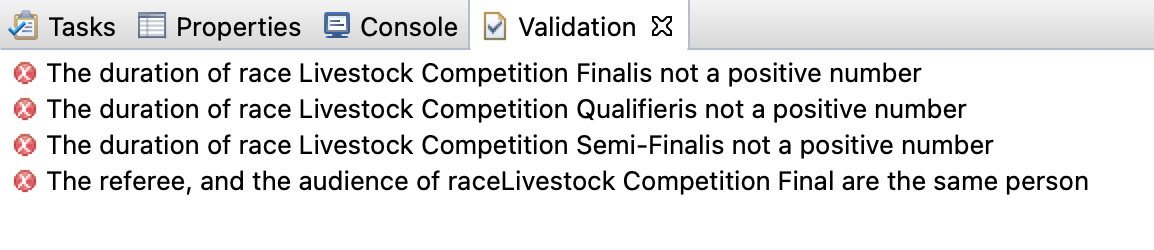
\includegraphics[scale = 0.6]{img/constraint-error}

\subsection{Integrating Constraints in Editor}
The author made the constraints integration mainly follow the step to step guide in the Epsilon Website, 
\href{https://www.eclipse.org/epsilon/doc/articles/evl-gmf-integration/}{Live validation and quick-fixes in GMF-based editors with EVL}.
There are the steps to make constraints integration in the graph editor, it is slightly different than the original post.
\begin{itemize}
    \item Create a evl file in the original editor.
    \item Right click StateFair, and select Plugin-in Tools, then open Manifest.
    \item In the dependencies, add org.eclipse.ui.ide and org.eclipse.epsilon.evl.emf.validation to the list of dependencies.
    \item In the extension, add org.eclipse.epsilon.evl.emf.validation. After that, right-click to add a new constraintBinding. 
    This is the step to tell the program to bind this project with the evl file which contains constraints. In the constraint* 
    field, browse the evl file, and select the directory of it. 
    \item Add the org.eclipse.ui.ide.markerResolution in extension, and right-click add generic script with following code.
    \newline class : org.eclipse.epsilon.evl.emf.validation.EvlMarkerResolutionGenerator
    \newline class : markerType : org.eclipse.emf.ecore.diagnostic
    \item Launch the project as a new instance, click the Edit, and select Validate 
\end{itemize}

\subsection{Integrated Constraints Errors}
After integrating constraints into the graph editor, in-editor errors or warnings can be displayed in the editor.

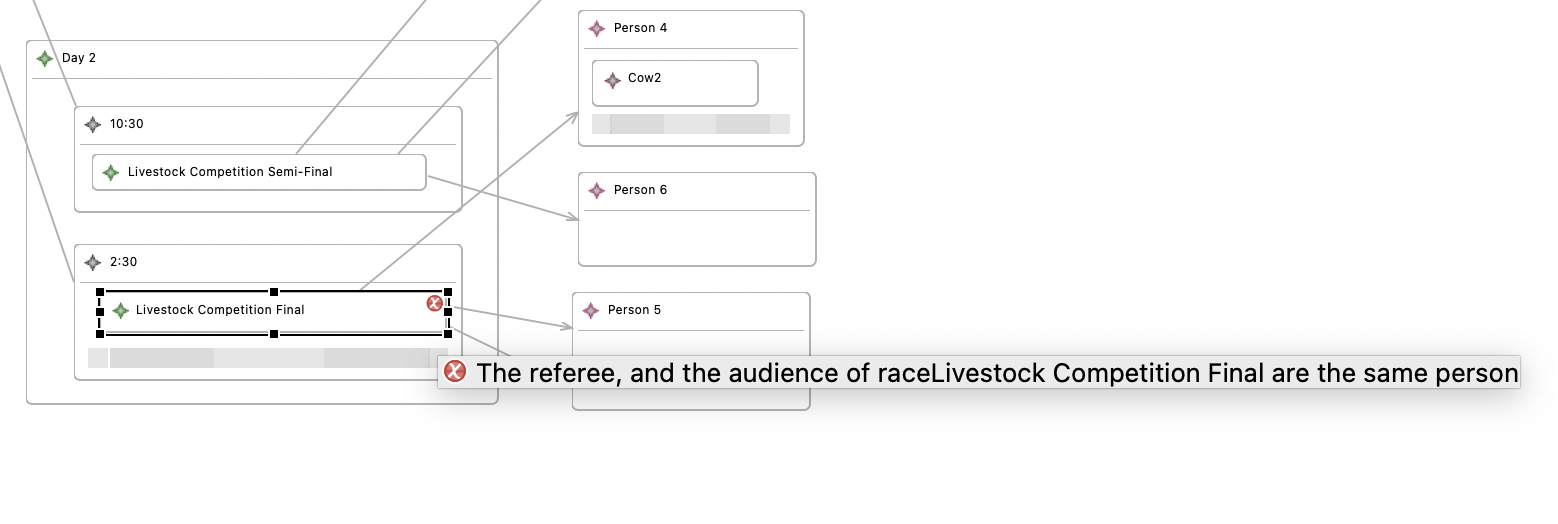
\includegraphics[scale = 0.6]{img/graph-editor-error1}

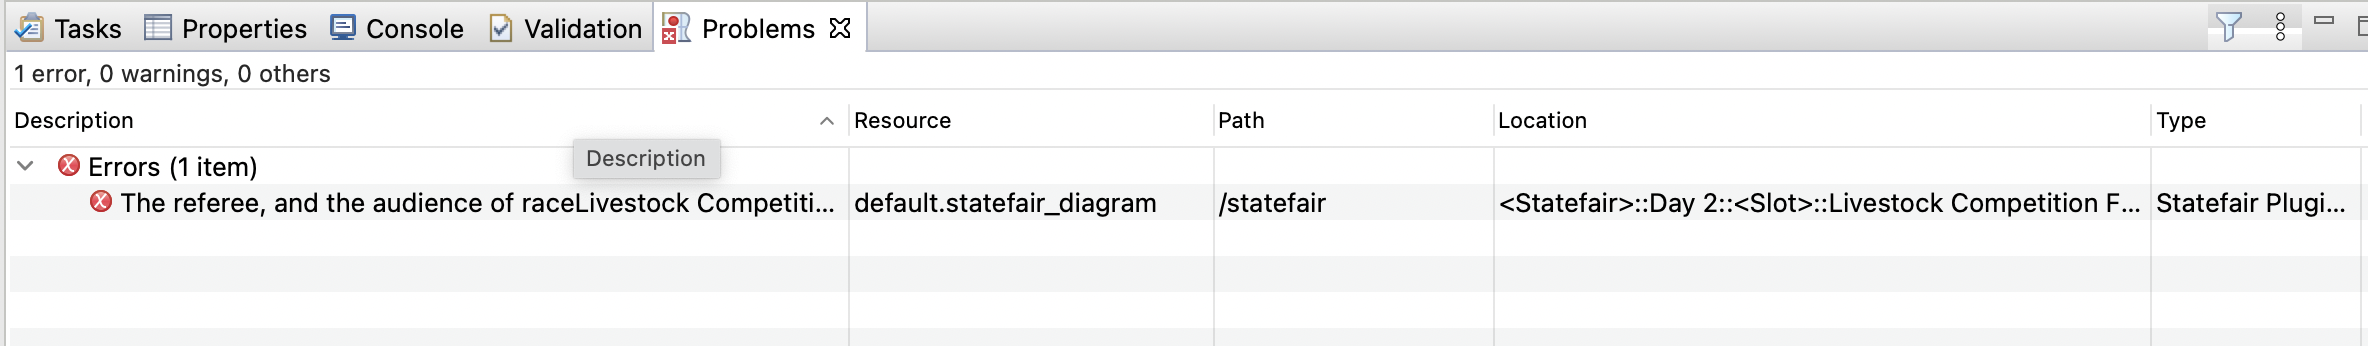
\includegraphics[scale = 0.4]{img/graph-editor-error2}

\subsection{Difficulties}
There are several unsolved problems in this project.

\begin{itemize}
    \item How to return the sum of the duration of observations and races? 
    \item How to get the total size of livestock in observations and races?
    \item One type of livestock may not get along with other types. For example, a male hog will 
    act aggressively if another male hog is nearby. In order to make the event more manageable, 
    the stalls need to be assigned base on certain rules. This will make things more complicated. 
    A new attribute, such as type, could be introduced to distinct animal types in the Animal 
    class. The Stall class has an attribute called location, this helps to indicate the stall location.
    \item The author tried to compare two times and determine which time is earlier time. The logic 
    could be using ":" as a delimiter, then compare the hour and minutes. The author runs some issues 
    with the program syntax, and not sure how and which way is the best to complete this task.
\end{itemize}

\pagebreak
\section{Model Transformation}
This model to text transformation is similar to the transformation presented in the lecture. However, the author expands the example 
and produces more complex html files to automate some work tasks. The following is what the html file will be generated.
\begin{itemize}
    \item The event schedule on each day. It contains the start time and end time, event name, duration, and who is the performer.
    \item An overall stall list. It contains the name of the stall, the size, and the location tag.
    \item The name badge of all participants in the state fair event.
\end{itemize}
~\newline
The implementation follows closely on the instruction of this tutorial - 
\href{https://www.eclipse.org/epsilon/doc/articles/code-generation-tutorial-egl/}{Code Generation Tutorial with EGL}

\subsection{Event Schedule}
An example of day 1 schedule.

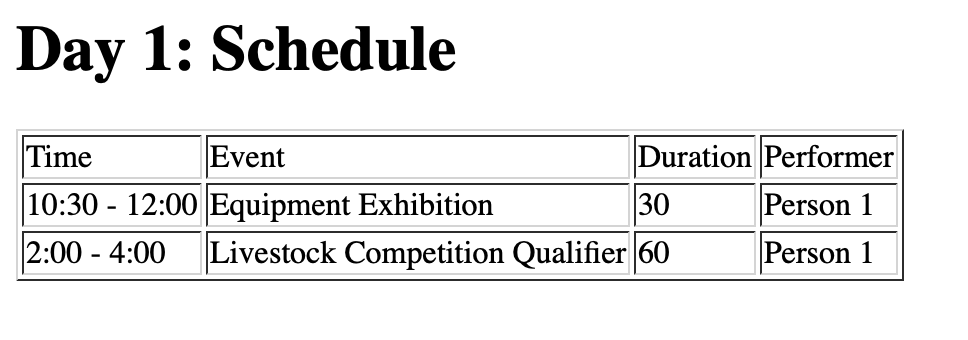
\includegraphics[scale = 0.6]{img/schedule}

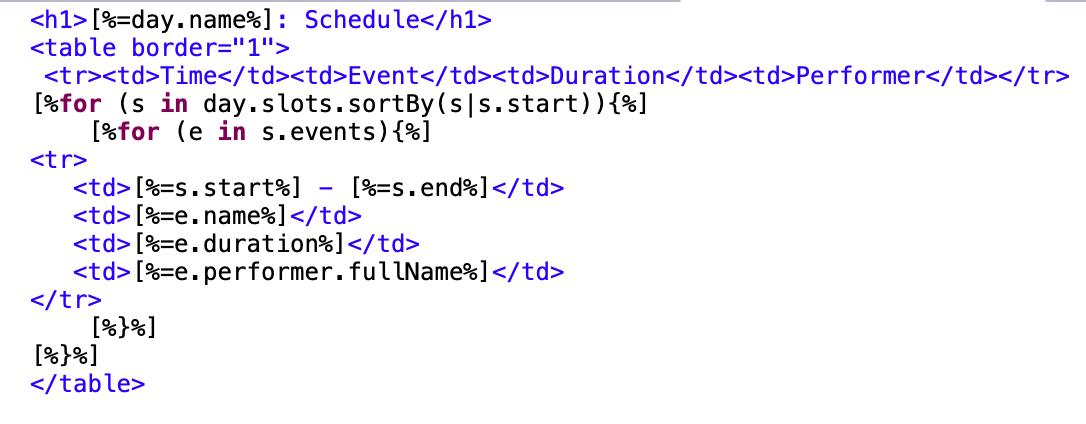
\includegraphics[scale = 0.6]{img/nestedloop}

\subsection{Whole Stall List}
An example of a list of all stalls.

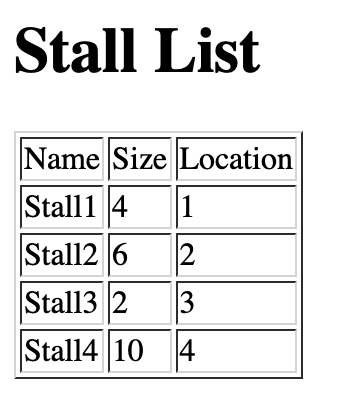
\includegraphics[scale = 0.6]{img/stall-list}

\subsection{Badge for each Individuals}
An example of a badge of a participant.

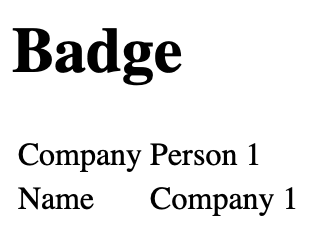
\includegraphics[scale = 0.6]{img/badge}

\subsection{Analysis}
The benefit of creating all different types of html files are enormous. From the practical view, it helps to keep the website, 
event booklets, and badge consistent. Moreover, it could save more time for a programmer to focus on other tasks, and save the 
company's resources in the long term.
\\
The author also thinks there should be some integration between the web server and Epsilon. For example, how the web server 
automatically picks up the right html file which generated by Epsilon, and updates it on the web page. Another integration 
is sending the name badge to each 
participant via email. Right now, the EGL model only can produce the name badge for all participants. An email bot may be needed 
to automatically send the badge html file to each individual.

\subsection{Difficulties}
There are some difficulties the author faced in the implementation. For example, how to print a list that only contains referees? 
Only Race class has the attribute of the referee, and the Race class is a child class of Event. When looping through 
the Event list, some instances can be Observation class which does not have an attribute of the referee.

\section{Summary}
Creating a DSL is an extremely interesting topic. The project demonstrates how to use Emfatic/Ecore to generate a class 
diagram of the metamodel, integrating a graph editor in Eugenia, adding validation constraints in the editor, and transforming 
the model to other forms. The report also provides opinions/insights on each implementation, include advantages, disadvantages, 
and difficulties.

\pagebreak
\section{Reference}
\begin{enumerate}
    \item \href{https://www.eclipse.org/epsilon/doc/articles/evl-gmf-integration/}{Live validation and quick-fixes in GMF-based editors with EVL}
    \item \href{https://www.eclipse.org/epsilon/doc/articles/code-generation-tutorial-egl/}{Code Generation Tutorial with EGL}
\end{enumerate}

\end {document}